\listfiles
\documentclass[fontsize=11pt,paper=a4,pagesize=auto]{report}

\usepackage{lmodern}
\usepackage[english]{babel}
\usepackage{blindtext}
\usepackage{microtype}
\usepackage{comment, subfiles, graphicx, caption, longtable, subfig, fancyhdr}
\usepackage{float} %Used to force image to appear in the section in which it's declared
\usepackage[hidelinks]{hyperref}
\usepackage[parfill]{parskip}
\usepackage[dvipsnames]{xcolor}
\usepackage{listings}
\usepackage{xurl}
\usepackage{geometry}

 \geometry{
 a4paper,
 total={170mm,257mm},
 left=20mm,
 top=20mm,
 }
\begin{document}

\begin{titlepage}
	\centering
	\bigskip
	\bigskip
	
\includegraphics[scale = 0.25]{images/polimi.jpg}\par
	
	{\scshape\Large
		Hypermedia Applications Project\\
		a.y. 2020-21\par}
			\vspace{0.5cm}
	{\huge\bfseries
	\bigskip
		Inspection and Usability Test Document\\\par}

	\vspace{0.5cm}
	{\Large
		{\scshape Bresciani} Matteo\\
		{\scshape D'Ascoli}  Gabriele\par

		}
			\vspace{1cm}

		{\huge\Large
		\bigskip
		Evaluated website:}\\
\bigskip
		
\includegraphics[scale = 0.30]{images/moviri-logo.png}\par
		
	
% Bottom of the page
\end{titlepage}

\tableofcontents
\chapter{Abstract}
The aim of this document is to report the Inspection-based Usability Evaluation and the User-Testing-based Usability Evaluation of Moviri website which can be found at the following url \url{https://www.moviri.com/}.  
\\
Into this document we analyze the website of Moviri, a multinational consulting and software group of companies, helping customers harness the power of transformative technologies; in the various sections the website shows the services offered to the clients: performance engineering, analytics, security and IoT. 
\\
In the Inspection section are reported the steps followed to reach the objective, the evaluation for the selected heuristics and examples to demonstrate the reason why certain ratings has been given. Then, in the User-Testing part are described the steps procedure that tester followed: 1. Execute given task following scenarios while they are evaluated with specific criteria 2. Surf the website freely 3. Fulfill a form with some questions related to landmarks, navigation and layout 

 

\part{Inspection}

\chapter{Overview}
In this part of the document we're focusing on the evaluation of usability of \textit{Moviri} through \textbf{inspection}. Inspection allow us to find usability issues and obstacles for the user when interacting with a web application. In particular, this is done thanks to \textbf{heuristics} which guide the expert to explore the website and check compliance with usability principles.
\section{Goals}
Before inspection, goals are defined in order to deeply inspect the website and to focus on the main aspect. 
\begin{itemize}
\item Read experiences of other companies and changes adopted;
\item Find the appropirate technology needed;
\item Interact with Moviri due to become a new customer;
\end{itemize}
\section{Inspection method}

We decide to adopt 2 different set of heuristics in order to inspect the website. 

\subsection{Mile's heuristics}
These heuristics are divided into different categories relevant to a particular aspect.

\textbf{Navigation}: It aims to evaluate the easiness with which an user navigates into each part of the website.
\begin{itemize} 
\item \textbf{Interaction consistency}: do pages of the same type have the same links and interaction capability?
\item \textbf{Group navigation}: is it easy to navigate from and among groups of
“items”?
\item \textbf{Structural Navigation}: is it easy to navigate among the semantic components of a Topic?
\item \textbf{Semantic Navigation}: is it easy to navigate among group members and from a group introductory page to group members (and the other way around)?
\item \textbf{Landmarks}: is it easy to navigate from a Topic to a related one?
\end{itemize}

\textbf{Contents}: It indicates how in the website information is well balanced in each page and section.  
\begin{itemize}
\item \textbf{Information Overload}: is the information in a page too much or too little and does it fit the page layout?
\end{itemize}

\textbf{Layout}: It serves to estimate if the website is graphically expressive enough and readable.
\begin{itemize}
\item \textbf{Text Layout}: is the text readable? Is font size appropriate?
\item \textbf{Interaction Placeholder-Semiotics}: are textual or visual labels of interactive elements “expressive”? i.e., do they reflect the meaning of the interaction and its effects? Are they consistent?
\item \textbf{Interaction Placeholders-Consistency}: are textual or visual labels of interactive elements consistent in terms of wording, icon, position, etc.?
\item \textbf{Spatial Allocation}: is the on-screen allocation of contents and visual appropriate for their relevance? Are “semantically related” elements close and “semantically distant” element far away?
\item \textbf{Consistency of Page Structure}: do pages of the same type have the same lay out (same visual properties of each component and similar lay-out organization of the various elements?)
\end{itemize} 

\subsection{Nielsen's heuristics}
These belongs to a set of 10 heuristics, which cover each aspect relevant for the evaluation. However, we decide not to evaluate every heuristic but only some of them. We decide this because in our opinion cannot be all classified in this website.
The heuristics are the following:
\begin{description} 
\item[1 -] \textbf{Visibility of system status}: the design should always keep users informed about what is going on, through appropriate feedback within a reasonable amount of time;
\item[2 -] \textbf{Match between system and the real world}: the design should speak the users' language. Use words, phrases, and concepts familiar to the user, rather than internal jargon. Follow real-world conventions, making information appear in a natural and logical order;
\item[4 -] \textbf{Consistency and standards}: users should not have to wonder whether different words, situations, or actions mean the same thing. Follow platform and industry conventions
\item[5 -] \textbf{Error prevention}: good error messages are important, but the best designs carefully prevent problems from occurring in the first place. Either eliminate error-prone conditions, or check for them and present users with a confirmation option before they commit to the action;
\item[7 -] \textbf{Flexibility and efficiency of use}: shortcuts — hidden from novice users — may speed up the interaction for the expert user such that the design can cater to both inexperienced and experienced users. Allow users to tailor frequent actions;
\item[8 -] \textbf{Aesthetic and minimalist design}: interfaces should not contain information which is irrelevant or rarely needed. Every extra unit of information in an interface competes with the relevant units of information and diminishes their relative visibility;
\end{description}


\section{Scoring metric}
Before the inspection, a metric is defined in order to evaluate each heuristic. The evaluation consist in the assigment of a score from 0 to 5. The following image gives an explanation of each score.

\begin{itemize}
\item \textbf{0}: The heuristics is not satisfied. Many severe violations are detected;;
\item \textbf{1}: The heuristics is not satisfied. Few severe violations are detected;
\item \textbf{2}: The heuristics is not satisfied because of relevant issues;
\item \textbf{3}: The heuristic is partially satisfied with some issues detected;
\item \textbf{4}: The heuristic is satisfied, but it can be improved;
\item \textbf{5}: No issue are detected. The heuristic is fully satisfied; 
\end{itemize} 

\chapter{Scores on each heuristics}
\section{Navigation}
\begin{table}[H]
  \begin{center}
    \label{tab:table1}
    \begin{tabular}{l|c|r} % <-- Alignments: 1st column left, 2nd middle and 3rd right, with vertical lines in between
      \textbf{Heuristic} & \textbf{Score} & \textbf{Comment}\\
      
      \hline
      Interaction Consistency & 1110.1 & a\\
      Group Navigation & 10.1 & b\\
      Structural Navigation & 23.113231 & c\\
      Semantic Navigation & 23.113231 & c\\
      Landmarks & 23.113231 & c\\

    \end{tabular}
  \end{center}
\end{table}

\subsection{Interaction Consistency}
The website offers a significant experience due to interaction. As a matter of fact, its structure is based on some elements available in each page:
\begin{itemize}
\item \textbf{Header}: it links to different pages. In particular it allow users to navigate on:
\begin{itemize}
\item Company's \textbf{social network profiles} (\textit{Facebook, Twitter, Instagram and Linkedin});
\item \textbf{News section} for incoming report regarding Moviri;
\item \textbf{Contact section} due to interact with Moviri's employees;
\item \textbf{Moviri Careers}. It's a secondary website of Moviri where there are informations regarding job oppurtunities (+ genaral description of lavorare con moviri);
\end{itemize}
\item \textbf{Topbar}: allows a user to surf in each section of the website. In addition provides a search function for any content; 
\item \textbf{Footer}: provides the same links to different sections of topbar and header, but at the foot of each page;
\end{itemize}
\subsection{Group Navigation}
Thanks to components such as topbar and footer, is possibile to navigate between each section through links. The fact that links are placed both high and low helps user's experience to be more intuitive.
\subsection{Structural Navigation}
Navigation along each page is easily feasible and understandable. Structural navigation change slightly between section.\\
For instance, in the \textit{Business Lines} section each topic is represented by the combination of image and description side by side and unpaired with respect to the next one.
While in the \textit{Resource} section each item is placed in a grid with its title and a respective image.  

\subsection{Semantic Navigation}
Navigation between pages of different sections is easily allowed by topbar and footer. Nevertheless, there are situations in which this is not reversible. In particular this is not possibile in the \textit{Resource} section after the click of an item. In fact, it redirects to pages of other websites leaving Moviri domain. It's sufficient to go back with the undo function of the browser, but could be quite uncomfortable.
\subsection{Landmarks}
These can be found both top and buttom part of the website in each section. It's always possibile to be redirect to the homepage. Anyway they could be improved to be more evident.

\section{Content}
\begin{table}[H]
  \begin{center}
    \label{tab:table1}
    \begin{tabular}{l|c|r} % <-- Alignments: 1st column left, 2nd middle and 3rd right, with vertical lines in between
      \textbf{Heuristic} & \textbf{Score} & \textbf{Comment}\\
      
      \hline
     Information Overload & 1110.1 & a\\
     
    \end{tabular}
  \end{center}
\end{table}
\subsection{Information Overload}
Each information, both graphical and textual, is well balanced in each section of the website. This is one of the strength of website.
\section{Layout}

\begin{table}[H]
  \begin{center}
    \label{tab:table1}
    \begin{tabular}{l|c|r} % <-- Alignments: 1st column left, 2nd middle and 3rd right, with vertical lines in between
      \textbf{Heuristic} & \textbf{Score} & \textbf{Comment}\\
      
      \hline
      Text Layout & 1110.1 & a\\
      Interaction Placeholder-Semiotics & 10.1 & b\\
      Interaction Placeholder-Consistency & 23.113231 & c\\
      Spatial Allocation & 23.113231 & c\\
      Consistency of Page Structure & 23.113231 & c\\

    \end{tabular}
  \end{center}
\end{table}

\subsection{Text Layout}
Textual contents are easy-to-read. This is thanks to the font used in each point which is always proportional to the importance of the information. For instance, title or quotes has a larger font then simple description. An other important aspect is the choice of the font colour. In fact this is always matched with the rest of the layout.
\subsection{Interaction Placeholder-Semiotics}
Textual and visual labels are expressive almost in every case. Only few situations link are not visible by underling or a hand-cursor. In addition we found relevant issues caracterized by a strange behaviour in some case. For instance, clicking on partners image in the \textit{Business Line} section, the page come back at the top of the page. Moreover, it happens that cliking on image TODO.
\subsection{Interaction Placeholder-Consistency}
Website is consistent due to its component such as wording, icon and position. In fact, due to the easiness of the website, this has no relevant issue.

\subsection{Spatial Allocation}
Each type of content is allocated spatially and semantically very well. 

\subsection{Consistency of Page Structure}
The layout in each page is generally the same, with few differences about contents allocation. Anyway, in the resource section users can be redirected to other websites with a completely different structure.\\
TODO


\chapter{Result and Discussion}
This section aims to join every results obtained in the last chapter in order to give a unique score for each heuristic section. This is done by computing the arithmetic average of the scores of \textit{Navigation}, \textit{Contents} and \textit{Layout} sections.\par
\bigskip
\section{Scores}
\subsection{MiLE}
\textbf{Navigation}\par
The navigation score is given by the mean of the 5 aspects analyzed in the section \ref{Navigation}. \par 
The final result is: 
(4.5 + 4.5 + 4 + 3.5 + 3.5)/5 = \textbf{4}\par
Therefore, content aspect in the Moviri website is handled well, even if could be improved again.

\begin{figure}[H]
  \centering
  \makebox[\linewidth]{
    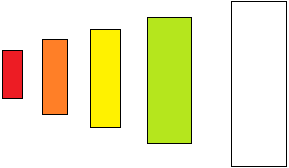
\includegraphics[scale=0.35]{images/4.png}}
\end{figure}

\par\medskip

\textbf{Contents}\par
The score of this section is given simply by the score evaluated by the \textit{Information Overload} heuristic which is \textbf{4.5}. \par
So basing only this heuristic, content of the website is almost fully satisfied. Improvements could be done, but fixes will be minimal.

\begin{figure}[H]
  \centering
  \makebox[\linewidth]{
    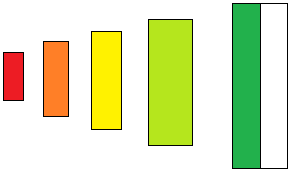
\includegraphics[scale=0.35]{images/4.5.png}}
\end{figure}


\par\medskip
\pagebreak
\textbf{Layout}\par
The layout score is given by the mean of 5 aspects analyzed in the section \ref{Layout}. \par
The final result is: 
(4 + 4 + 4 + 4 + 3)/5 = 3.8 \\
\textit{which can be approximated to} \textbf{4}\par
Basing on the result, layout of the website it's pretty well designed, but with some critical issues that should be fixed in order to have the best experience.

\begin{figure}[H]
  \centering
  \makebox[\linewidth]{
    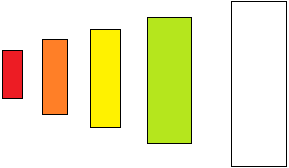
\includegraphics[scale=0.35]{images/4.png}}
\end{figure}


\subsection{Nielsen}
Instead, the evaluation with this set of heuristics is made by making the average of all the six heuristcs analyzed:
(2 + 4 + 3.5 + 4 + 5 + 4.5)/6 = 3.8 \\
\textit{which can be approximated to} \textbf{4}.\par

\begin{figure}[H]
  \centering
  \makebox[\linewidth]{
    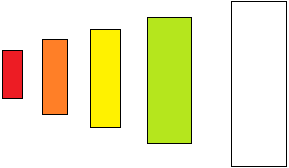
\includegraphics[scale=0.35]{images/4.png}}
\end{figure}

\section{Comments}
As evidenced by the results obtained from the analysis carried out by our team, the site has high standards obtained on the various fields evaluated and, although there are criticalities widely described in the appropriate sections, as a whole it is functional, well done and adequate for its purpose of use; our work concerning the Inspection of the web site therefore ends with an overall satisfactory score.


\part{Usability Test}

\chapter{Overview}
In this part of the document we evaluate usability of Moviri basing on \textbf{User Testing}. User testing is a technique based on user-experience used to evaluate a product by testing it on selected users. Instead of inspection, this is more focused on human–computer interaction in order to eveluate the easyness of a website.

\section{Design of the study}
\subsection{User Profile}
User profile definition is very relevant for user testing. In fact, this help us to understand who can be recruited for user testing. The user profile detected are the following:

\medskip
\textbf{Profile 1}\par
\begin{itemize}
\item \textit{Age}: between 25 and 30 years old;
\item \textit{Civil state}: irrelevant;
\item \textit{Technology capabilities}: General knowledge about Computer Science;
\end{itemize}

\medskip
\textbf{Profile 2}\par
\begin{itemize}
\item \textit{Age}: between 40 and 50 years old;
\item \textit{Civil state}: irrelevant;
\item \textit{Technology capabilities}: Simple web user with any particular capabilities;
\end{itemize}

\subsection{Scenarios}
In this subsection are shown the goals of the user testing followed by the tasks needed to reach them:\par
\textbf{Scenario 1}: You need a job and you know that Moviri has a lots of open positions. You’re applying for a job opportunity.
\begin{enumerate}
\item Visit the website section for career service;
\item Start the application procedure;
\item Choose a type of job offer that is suitable for your background (such as Software Engineering); 
\item Select the position for which you want to run for;
\item Insert your data in the form for the application;
\item Turn to the homepage;
\end{enumerate}\par
\textbf{Scenario 2}: you’re looking for a white paper related to a particular service/solution for your company.
\begin{enumerate}
\item Visit the website section for consulting Moviri’s resource;
\item Find and select the white paper that you need;
\item Fill out the form with your information in order to receive the white paper by e-mail;
\item Turn to the homepage;
\end{enumerate}\par
\textbf{Scenario 3}: you’re looking for a initiative called “Keep IT Up” and you want to keep current on it.
\begin{enumerate}
\item Visit the website section relevant to news;
\item Find the article about “Keep IT Up” initiative and select it;
\item After you get some info from the article, in order to stay up fill out the form;
\end{enumerate}\par

\subsection{Variable Measure}
In order to evaluate user testing on some metrics, usability variables are defined:
\begin{itemize}
\item \textbf{Time of execution}: it's measure in \textit{seconds} and represents the time spent on a given task. It starts from the moment in which user begin focusing his attention on it;
\item \textbf{Effectiveness}: it represents the task success rate. It's measured by a value \textbf{between 0 and 1}:
    \begin{itemize} 
    \item \textit{1.0}: task completed with success;
    \item \textit{0.5}: task partially completed;
    \item \textit{0.0}: task is not completed;
    \end{itemize}
\item \textbf{Errors}: it's measured by an integer representing the number of errors made during the execution on a given task;
\item \textbf{Perceived tasks difficulty}: it's expressed by an integer \textit{between 0 and 5} given by an user after the completion of a given task;
\item \textbf{Satisfaction}: it's given by an integer \textit{between 0 and 5} provided by user immediately after the task execution;
\end{itemize}


\subsection{Final Survey}
After the execution of every tasks, a final survey is provided to users in order to have additional collected data. This provides extra feedbacks about aspects already highlighted during the inspection.
The questions, provided through a survey made with Google Forms at the link \url{www.ciao.123}, are the following:
\begin{enumerate}
\item Did you find virtual design intuitive and consistent?
\item Did you find images dimension good and well positioned?
\item Did you find the navigation between each sections appropriate?
\item How much easy was to navigate between different website domains due to task completion?
\item How much easy was to find landmarks?
\item How much easy was to carry out each task (in general)?
\end{enumerate}

\chapter{Execution of the study}
In this section are attached the values sampled during the the execution of the user testing. In particular, 5 user was choosen for this user testing.

\section{Hardware and Software settings}
The study was executed using laptops by each user. There are no other type of hardware components used to make this test.
Instead, for the software side we adopt \textit{Microsoft Teams} in order to perform tests remotely. In this way, each variable has been evaluated directly using a \textit{task sheet}.
\section{Evaluations}
Here it's possible to look at the results collected in tables, one for each user involved in the test.

\subsection{Profile 1}
\begin{table}[H]
  \begin{center}
    \label{tab:table1}
    \begin{tabular}{||c|c|c|c|c|c||} % <-- Alignments: 1st column left, 2nd middle and 3rd right, with vertical lines in between
      \textbf{Scenario} & \textbf{Task} & \textbf{Time Execution} & \textbf{Effectivness} & \textbf{Error} & \textbf{Satisfaction}\\
      
      \hline
        1 & 1 & 9 & 1 & 0 & 5\\
        1 & 2 & 8 & 1 & 0 & 5\\
        1 & 3 & 10 & 1 & 0 & 5\\
        1 & 4 & 5 & 1 & 0 & 5\\
        1 & 5 & 42 & 1 & 0 & 5\\
        1 & 6 & 6 & 1 & 0 & 4\\
        \hline
        2 & 1 & 10 & 1 & 0 & 4\\
        2 & 2 & 14 & 1 & 0 & 5\\
        2 & 3 & 32 & 1 & 0 & 5\\
        2 & 4 & 10 & 1 & 0 & 4\\
        \hline
        3 & 1 & 10 & 1 & 0 & 5\\
        3 & 2 & 23 & 1 & 0 & 4\\
        3 & 3 & 42 & 1 & 0 & 5\\
        \hline

    \end{tabular}
  \end{center}
  \caption{User ID 01 (Profile 1)}
\end{table}

\begin{table}[H]
  \begin{center}
    \label{tab:table1}
    \begin{tabular}{||c|c|c|c|c|c||} % <-- Alignments: 1st column left, 2nd middle and 3rd right, with vertical lines in between
      \textbf{Scenario} & \textbf{Task} & \textbf{Time Execution} & \textbf{Effectivness} & \textbf{Error} & \textbf{Satisfaction}\\
      
      \hline
        1 & 1 & 14 & 1 & 0 & 5\\
        1 & 2 & 3 & 1 & 0 & 5\\
        1 & 3 & 25 & 1 & 0 & 5\\
        1 & 4 & 13 & 1 & 0 & 5\\
        1 & 5 & 44 & 1 & 0 & 5\\
        1 & 6 & 31 & 1 & 1 & 2\\
        \hline
        2 & 1 & 5 & 1 & 0 & 5\\
        2 & 2 & 23 & 1 & 0 & 5\\
        2 & 3 & 28 & 1 & 0 & 5\\
        2 & 4 & 5 & 1 & 0 & 5\\
        \hline
        3 & 1 & 7 & 1 & 0 & 5\\
        3 & 2 & 23 & 1 & 0 & 5\\
        3 & 3 & 31 & 1 & 0 & 5\\
        \hline

    \end{tabular}
  \end{center}
  \caption{User ID 02 (Profile 1)}
\end{table}

\begin{table}[H]
  \begin{center}
    \label{tab:table1}
    \begin{tabular}{||c|c|c|c|c|c||} % <-- Alignments: 1st column left, 2nd middle and 3rd right, with vertical lines in between
      \textbf{Scenario} & \textbf{Task} & \textbf{Time Execution} & \textbf{Effectivness} & \textbf{Error} & \textbf{Satisfaction}\\
      
      \hline
        1 & 1 & 11 & 1 & 0 & 5\\
        1 & 2 & 6 & 1 & 0 & 5\\
        1 & 3 & 17 & 1 & 0 & 5\\
        1 & 4 & 9 & 1 & 0 & 5\\
        1 & 5 & 43 & 1 & 0 & 5\\
        1 & 6 & 19 & 1 & 0 & 4\\
        \hline
        2 & 1 & 8 & 1 & 0 & 5\\
        2 & 2 & 19 & 1 & 0 & 5\\
        2 & 3 & 30 & 1 & 0 & 4\\
        2 & 4 & 8 & 1 & 0 & 5\\
        \hline
        3 & 1 & 9 & 1 & 0 & 5\\
        3 & 2 & 23 & 1 & 0 & 4\\
        3 & 3 & 35 & 1 & 0 & 5\\
        \hline

    \end{tabular}
  \end{center}
  \caption{User ID 03 (Profile 1)}
\end{table}

\begin{table}[H]
  \begin{center}
    \label{tab:table1}
    \begin{tabular}{||c|c|c|c|c|c||} % <-- Alignments: 1st column left, 2nd middle and 3rd right, with vertical lines in between
      \textbf{Scenario} & \textbf{Task} & \textbf{Time Execution} & \textbf{Effectivness} & \textbf{Error} & \textbf{Satisfaction}\\
      
      \hline
        1 & 1 & 12 & 1 & 0 & 5\\
        1 & 2 & 13 & 1 & 0 & 5\\
        1 & 3 & 11 & 1 & 0 & 5\\
        1 & 4 & 8 & 1 & 0 & 5\\
        1 & 5 & 25 & 1 & 0 & 5\\
        1 & 6 & 13 & 1 & 0 & 4\\
        \hline
        2 & 1 & 12 & 1 & 0 & 5\\
        2 & 2 & 11 & 1 & 0 & 5\\
        2 & 3 & 29 & 1 & 0 & 5\\
        2 & 4 & 11 & 1 & 0 & 5\\
        \hline
        3 & 1 & 15 & 1 & 0 & 5\\
        3 & 2 & 23 & 1 & 0 & 4\\
        3 & 3 & 22 & 1 & 0 & 5\\
        \hline

    \end{tabular}
  \end{center}
  \caption{User ID 04 (Profile 1)}
\end{table}


\begin{table}[H]
  \begin{center}
    \label{tab:table1}
    \begin{tabular}{||c|c|c|c|c|c||} % <-- Alignments: 1st column left, 2nd middle and 3rd right, with vertical lines in between
      \textbf{Scenario} & \textbf{Task} & \textbf{Time Execution} & \textbf{Effectivness} & \textbf{Error} & \textbf{Satisfaction}\\
      
      \hline
        1 & 1 & 12 & 1 & 0 & 5\\
        1 & 2 & 10 & 1 & 0 & 5\\
        1 & 3 & 14 & 1 & 0 & 5\\
        1 & 4 & 9 & 1 & 0 & 5\\
        1 & 5 & 34 & 1 & 0 & 5\\
        1 & 6 & 16 & 1 & 0 & 4\\
        \hline
        2 & 1 & 9 & 1 & 0 & 5\\
        2 & 2 & 15 & 1 & 0 & 5\\
        2 & 3 & 29 & 1 & 0 & 5\\
        2 & 4 & 9 & 1 & 0 & 5\\
        \hline
        3 & 1 & 12 & 1 & 0 & 5\\
        3 & 2 & 22 & 1 & 0 & 5\\
        3 & 3 & 31 & 1 & 0 & 5\\
        \hline

    \end{tabular}
  \end{center}
  \caption{User ID 05 (Profile 1)}
\end{table}


\subsection{Profile 2}

\begin{table}[H]
  \begin{center}
    \label{tab:table1}
    \begin{tabular}{||c|c|c|c|c|c||} % <-- Alignments: 1st column left, 2nd middle and 3rd right, with vertical lines in between
      \textbf{Scenario} & \textbf{Task} & \textbf{Time Execution} & \textbf{Effectivness} & \textbf{Error} & \textbf{Satisfaction}\\
      
      \hline
        1 & 1 & 40 & 1 & 0 & 3\\
        1 & 2 & 5 & 1 & 0 & 5\\
        1 & 3 & 40 & 0.5 & 0 & 5\\
        1 & 4 & 7 & 1 & 0 & 5\\
        1 & 5 & 40 & 1 & 0 & 5\\
        1 & 6 & 45 & 0.5 & 1 & 3\\
        \hline
        2 & 1 & 13 & 1 & 0 & 5\\
        2 & 2 & 23 & 1 & 0 & 5\\
        2 & 3 & 30 & 1 & 0 & 5\\
        2 & 4 & 74 & 0 & 2 & 2\\
        \hline
        3 & 1 & 30 & 1 & 0 & 5\\
        3 & 2 & 5 & 1 & 0 & 5\\
        3 & 3 & 33 & 1 & 0 & 5\\
        \hline

    \end{tabular}
  \end{center}
  \caption{User ID 06 (Profile 2)}
\end{table}

\begin{table}[H]
  \begin{center}
    \label{tab:table1}
    \begin{tabular}{||c|c|c|c|c|c||} % <-- Alignments: 1st column left, 2nd middle and 3rd right, with vertical lines in between
      \textbf{Scenario} & \textbf{Task} & \textbf{Time Execution} & \textbf{Effectivness} & \textbf{Error} & \textbf{Satisfaction}\\
      
      \hline
        1 & 1 & 15 & 1 & 0 & 5\\
        1 & 2 & 12 & 1 & 0 & 5\\
        1 & 3 & 27 & 0.5 & 0 & 5\\
        1 & 4 & 6 & 1 & 0 & 4\\
        1 & 5 & 25 & 1 & 0 & 4\\
        1 & 6 & 26 & 1 & 0 & 5\\
        \hline
        2 & 1 & 17 & 1 & 0 & 5\\
        2 & 2 & 34 & 1 & 0 & 3\\
        2 & 3 & 28 & 1 & 1 & 4\\
        2 & 4 & 11 & 1 & 1 & 5\\
        \hline
        3 & 1 & 14 & 1 & 0 & 5\\
        3 & 2 & 42 & 0.5 & 0 & 3\\
        3 & 3 & 48 & 1 & 0 & 5\\
        \hline

    \end{tabular}
  \end{center}
  \caption{User ID 07 (Profile 2)}
\end{table}

\begin{table}[H]
  \begin{center}
    \label{tab:table1}
    \begin{tabular}{||c|c|c|c|c|c||} % <-- Alignments: 1st column left, 2nd middle and 3rd right, with vertical lines in between
      \textbf{Scenario} & \textbf{Task} & \textbf{Time Execution} & \textbf{Effectivness} & \textbf{Error} & \textbf{Satisfaction}\\
      
           \hline
        1 & 1 & 25 & 1 & 0 & 4\\
        1 & 2 & 9 & 1 & 0 & 5\\
        1 & 3 & 32 & 1 & 0 & 5\\
        1 & 4 & 7 & 1 & 0 & 5\\
        1 & 5 & 40 & 1 & 0 & 5\\
        1 & 6 & 32 & 1 & 1 & 3\\
        \hline
        2 & 1 & 5 & 1 & 0 & 5\\
        2 & 2 & 28 & 1 & 0 & 5\\
        2 & 3 & 24 & 1 & 0 & 5\\
        2 & 4 & 35 & 0 & 1 & 2\\
        \hline
        3 & 1 & 23 & 1 & 1 & 3\\
        3 & 2 & 34 & 1 & 0 & 5\\
        3 & 3 & 32 & 1 & 0 & 5\\
        \hline
    \end{tabular}
  \end{center}
  \caption{User ID 08 (Profile 2)}
\end{table}

\begin{table}[H]
  \begin{center}
    \label{tab:table1}
    \begin{tabular}{||c|c|c|c|c|c||} % <-- Alignments: 1st column left, 2nd middle and 3rd right, with vertical lines in between
      \textbf{Scenario} & \textbf{Task} & \textbf{Time Execution} & \textbf{Effectivness} & \textbf{Error} & \textbf{Satisfaction}\\
      
      \hline
        1 & 1 & 13 & 1 & 0 & 4\\
        1 & 2 & 11 & 1 & 0 & 4\\
        1 & 3 & 26 & 0.5 & 1 & 4\\
        1 & 4 & 6 & 1 & 0 & 5\\
        1 & 5 & 24 & 1 & 0 & 5\\
        1 & 6 & 20 & 1 & 0 & 5\\
        \hline
        2 & 1 & 16 & 1 & 0 & 4\\
        2 & 2 & 31 & 1 & 0 & 4\\
        2 & 3 & 22 & 0.5 & 1 & 4\\
        2 & 4 & 18 & 1 & 0 & 5\\
        \hline
        3 & 1 & 13 & 1 & 0 & 5\\
        3 & 2 & 38 & 1 & 0 & 5\\
        3 & 3 & 47 & 1 & 0 & 3\\
        \hline

    \end{tabular}
  \end{center}
  \caption{User ID 09 (Profile 2)}
\end{table}


\begin{table}[H]
  \begin{center}
    \label{tab:table1}
    \begin{tabular}{||c|c|c|c|c|c||} % <-- Alignments: 1st column left, 2nd middle and 3rd right, with vertical lines in between
      \textbf{Scenario} & \textbf{Task} & \textbf{Time Execution} & \textbf{Effectivness} & \textbf{Error} & \textbf{Satisfaction}\\
      
        \hline
        1 & 1 & 32 & 1 & 1 & 3\\
        1 & 2 & 11 & 1 & 0 & 4\\
        1 & 3 & 26 & 1 & 1 & 4\\
        1 & 4 & 6 & 1 & 0 & 5\\
        1 & 5 & 24 & 1 & 0 & 5\\
        1 & 6 & 20 & 1 & 1 & 5\\
        \hline
        2 & 1 & 18 & 1 & 0 & 5\\
        2 & 2 & 25 & 1 & 0 & 5\\
        2 & 3 & 28 & 0.5 & 1 & 5\\
        2 & 4 & 18 & 1 & 0 & 5\\
        \hline
        3 & 1 & 11 & 1 & 0 & 5\\
        3 & 2 & 33 & 1 & 0 & 5\\
        3 & 3 & 26 & 1 & 0 & 4\\
        \hline

    \end{tabular}
  \end{center}
  \caption{User ID 10 (Profile 2)}
\end{table}

\chapter{Result Usability test}
\section{Usability test}
Here are shown the results of the previous sections aggregated making the average of the values for each different user profile:

\subsection{Profile 1}
\begin{table}[H]
  \begin{center}
    \begin{tabular}{||c|c|c|c|c|c||} % <-- Alignments: 1st column left, 2nd middle and 3rd right, with vertical lines in between
      \textbf{Scenario} & \textbf{Task} & \textbf{Time Execution} & \textbf{Effectivness} & \textbf{Error} & \textbf{Satisfaction}\\
      
      \hline
        1 & 1 & 9 & 1 & 0 & 5\\
        1 & 2 & 8 & 1 & 0 & 5\\
        1 & 3 & 10 & 1 & 0 & 5\\
        1 & 4 & 5 & 1 & 0 & 5\\
        1 & 5 & 30 & 1 & 0 & 5\\
        1 & 6 & 6 & 1 & 0 & 5\\
        \hline
        2 & 1 & 10 & 1 & 0 & 4\\
        2 & 2 & 14 & 1 & 0 & 5\\
        2 & 3 & 32 & 1 & 0 & 5\\
        2 & 4 & 10 & 1 & 0 & 5\\
        \hline
        3 & 1 & 10 & 1 & 0 & 5\\
        3 & 2 & 23 & 1 & 0 & 5\\
        3 & 3 & 42 & 1 & 0 & 5\\
        \hline

    \end{tabular}
  \end{center}
  \caption{Average results of Profile 1}
\end{table}

\subsection{Profile 2}


\begin{table}[H]
  \begin{center}
    \begin{tabular}{||c|c|c|c|c|c||} % <-- Alignments: 1st column left, 2nd middle and 3rd right, with vertical lines in between
      \textbf{Scenario} & \textbf{Task} & \textbf{Time Execution} & \textbf{Effectivness} & \textbf{Error} & \textbf{Satisfaction}\\
      
      \hline
        1 & 1 & 9 & 1 & 0 & 5\\
        1 & 2 & 8 & 1 & 0 & 5\\
        1 & 3 & 10 & 1 & 0 & 5\\
        1 & 4 & 5 & 1 & 0 & 5\\
        1 & 5 & 30 & 1 & 0 & 5\\
        1 & 6 & 6 & 1 & 0 & 5\\
        \hline
        2 & 1 & 10 & 1 & 0 & 4\\
        2 & 2 & 14 & 1 & 0 & 5\\
        2 & 3 & 32 & 1 & 0 & 5\\
        2 & 4 & 10 & 1 & 0 & 5\\
        \hline
        3 & 1 & 10 & 1 & 0 & 5\\
        3 & 2 & 23 & 1 & 0 & 5\\
        3 & 3 & 42 & 1 & 0 & 5\\
        \hline

    \end{tabular}
  \end{center}
  \caption{Average results of Profile 2}
\end{table}

\subsection{Total Average}
\begin{figure}[H]
  \centering
  \makebox[\linewidth]{
    
\includegraphics[scale=0.35]{images/averages.png}}
\end{figure}


\subsection{Survey results}

\subsection{Comment}






\chapter{Conclusion}
Regarding the first part of the \textit{Inspection}, as this usability evaluation study has highlighted, the Moviri’s website gives to users a quite good experience that could be easily improved by solving the found small issues.\\ 
For what concern Navigation, the strength is given by the Structural and Group Navigation:
\begin{itemize}
\item ensure a consistent aspect between pages; 
\item give an intuitive way to navigate between contents; 
\item overcome all navigation problems related to links’ miss between contents of a same; topic and structural problems. This aspect could be better managed by adding the possibility to go back to previous page (for example by including the followed path to reach each page); by adding links and letting users to move between similar contents without always accessing the header and by being more consistent in buttons layout and and visibility (for example by always showing only the one related to the selected season).
\end{itemize}
Content have taken the best score between the 4 groups because the website contains lots of information well organized and without visible issues. The only adjustments that could be done is that sometimes the layout was found a little too rough but with a small effort could make pages look tidier and more clear.\\
The real Presentation weak point is given by the lack of consistency between the pages of different groups, first, and of the placeholders, not always consistent and that can be easily improved.\\
Regarding Nielsen’s Heuristics the strenght point is the Efficiency of use, in fact we would like to say that the site is well done and ensures the user a good quality of the visit; the weak point, instead, is the visibility of the system status that is really lacking and demonstrates how much the developers have thought of a specialized user profile that has no problem finding himself in the various sections he wants to visit.
\par
Regarding the second part of the study, that concerns the \textit{User Testing}, we have already discussed into the results section the issued encountered by our testers but as conclusion we can say that our testers appreciated the website in its structure, layout and graphical elements and that they didn’t face big issues.\\
An evidence that we found both in the testers coming from Profile 1 and 2 regards the difficulty in identifying the landmark for the \textit{“Home”} section; as already underlined in the specific section of the system, this role is covered by \textit{"Business Lines"} button but without this being specified in any way, which leaves the user perplexed at first.\\
At the end, a suggestion that we can formulate by the analysis of all the data obtained by the study is that how as we had already seen, the web site can be easily consulted by a skilled user in the IT sector and becomes less and less easily visited by less experienced users for the complexity of the language that is used; we believe that these characteristics are predictable in a site that presents sectorial services and topics, designed for a well-defined user profile but some precautionsalready mentioned previously, such as the use of labels that clarify and anticipate the content of each section, could certainly make it usable to a much wider range of users.\\
We encounter some difficulties in alligning our ways of reasoning over the analyzed aspects and also in getting the heuristics limits.\par 
We found this project kinda complex but in the same time interesting because it allowed us to understand in a clear way what has an impact over our sentiment as users and how we would like a website to be done.


\appendix
\chapter{Annex}
The following tables are the ones from which we had computed each heuristics value.

\begin{table}[H]
  \begin{center}
    \begin{tabular}{|l|c|c|} % <-- Alignments: 1st column left, 2nd middle and 3rd right, with vertical lines in between
          \hline

      \textbf{Heuristic} & \textbf{Matteo} & \textbf{Gabriele}\\
      
      \hline
      Interaction Consistency & 5 & 4\\
      \hline
      Group Navigation & 4 & 5\\
      \hline
      Structural Navigation & 4 & 4\\
      \hline
      Semantic Navigation & 4 & 3\\
      \hline
      Landmarks & 3 & 4\\
    \hline 
    \hline
    \hline

     Information Overload & 5 & 4\\
    \hline 
    \hline
    \hline
     Text Layout & 4 & 4\\
      \hline
      Interaction Placeholder-Semiotics & 4 & 4\\
      \hline
      Interaction Placeholder-Consistency & 5 & 3\\
      \hline
      Spatial Allocation & 4 & 4\\
      \hline
      Consistency of Page Structure & 2 & 4\\

\hline
    \end{tabular}
  \end{center}
\end{table}


\end{document}